\documentclass{sa}
\usepackage{array} %dla poziomego wyrownania (m) w tabeli
\usepackage{soul}

\newcommand{\ang}[1]{(ang. \emph{#1})}
\renewcommand{\vec}[1]{\ensuremath\mathbf{#1}}
\newcommand{\grad}{\ensuremath\nabla}
\let\avg\overline

\usetikzlibrary{datavisualization}
\usetikzlibrary{datavisualization.formats.functions}

\usepackage{hyperref}
\graphicspath{{04_klasyfikacja/}}
\subtitle{Klasyfikacja}
\begin{document}
\begin{frame}
\titlepage
\end{frame}

\begin{frame}{Klasyfikacja}
\begin{block}{Zadanie klasyfikacji binarnej}
Dla danego wektora cech $\vec{x}$ opisującego obiekt przewidzieć czy obiekt należy do klasy \emph{pozytywnej} $y=1$ czy \emph{negatywnej} $y=0$ (lub $y=-1$).
\end{block}
\end{frame}

\begin{frame}{Irysy}
Pomarańczowy: Iris Virginica, niebieski: pozostałe
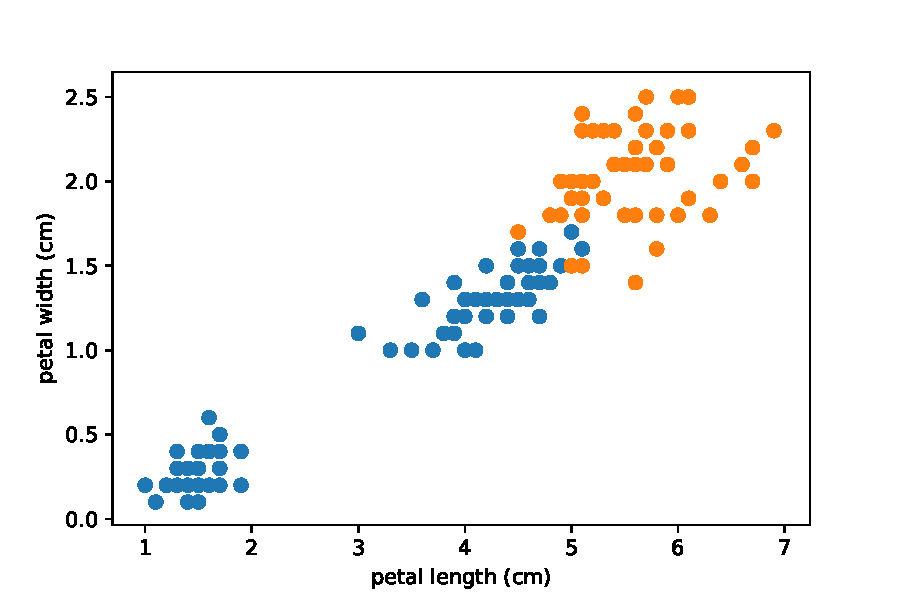
\includegraphics[width=\textwidth]{iris-simplified.pdf}
\end{frame}

\begin{frame}{Przewidywanie prawdopodobieństwa -- regresja liniowa}
Punkty w tle: prawd. Iris Virginica (jaśniej=wyższe)
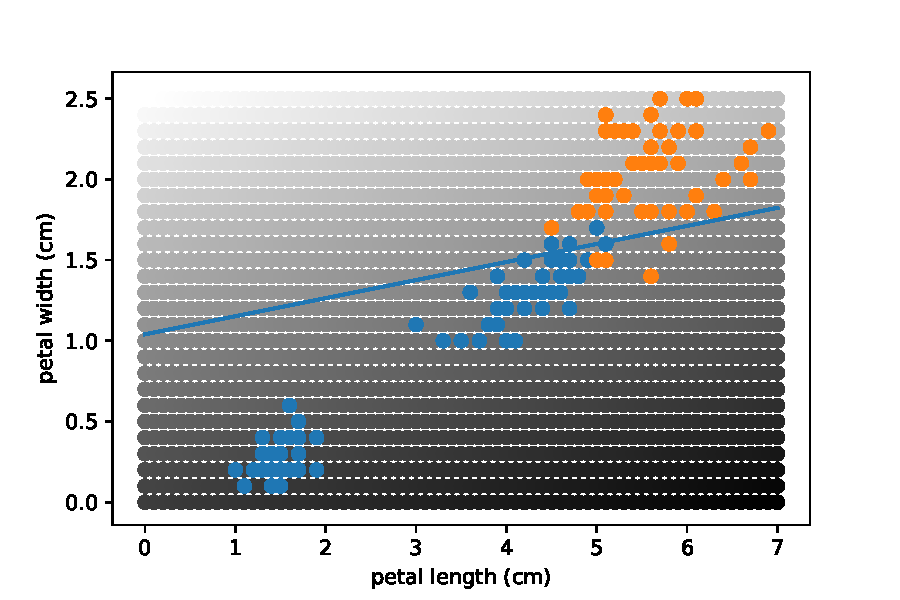
\includegraphics[width=\textwidth]{iris-simplified-linreg.pdf}
\end{frame}

\begin{frame}{Przewidywanie prawdopodobieństwa -- regresja logistyczna}
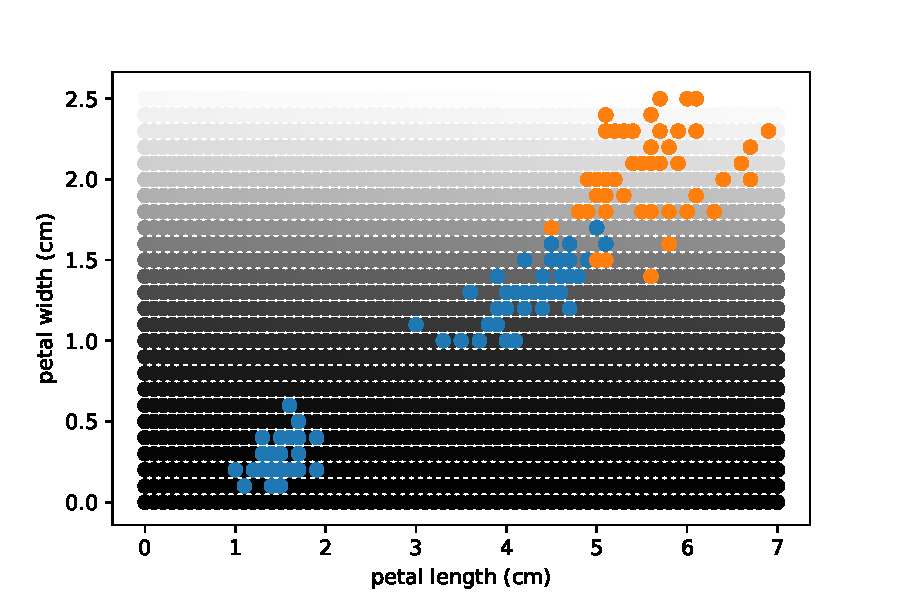
\includegraphics[width=\textwidth]{iris-simplified-logreg.pdf}
\end{frame}

\begin{frame}{Granica decyzyjna (ang. decision boundary)}
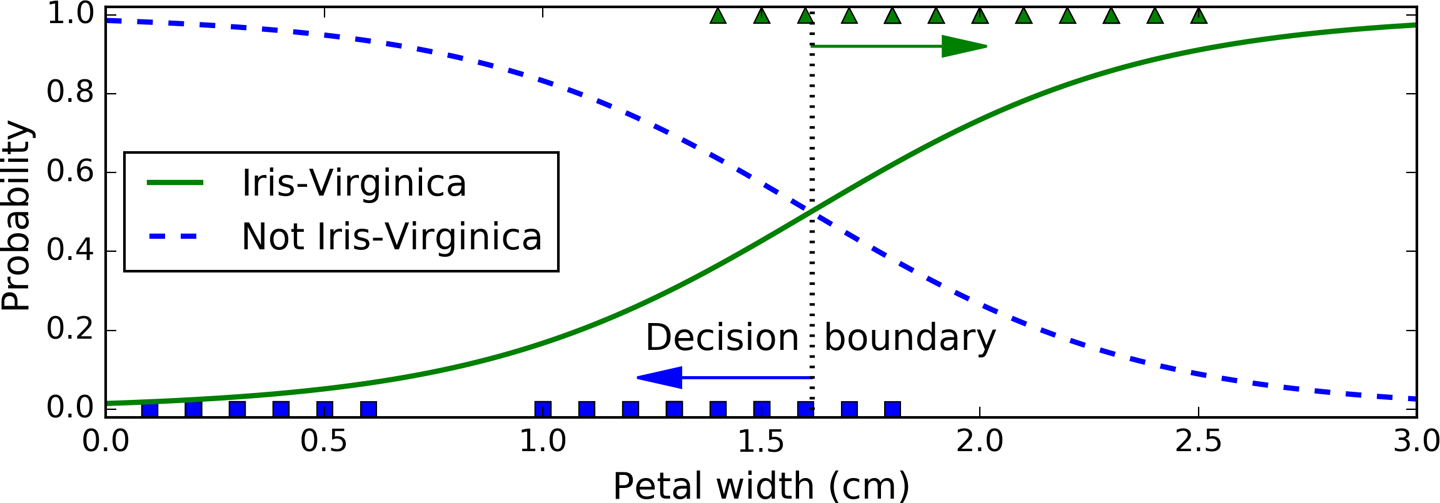
\includegraphics[width=\textwidth]{iris-1attr-decboundary.png}
{\vfill\footnotesize A. Géron, \emph{Hands-On Machine Learning with Scikit-Learn and TensorFlow} 2017}
\end{frame}

\begin{frame}{Granica decyzyjna (ang. decision boundary)}
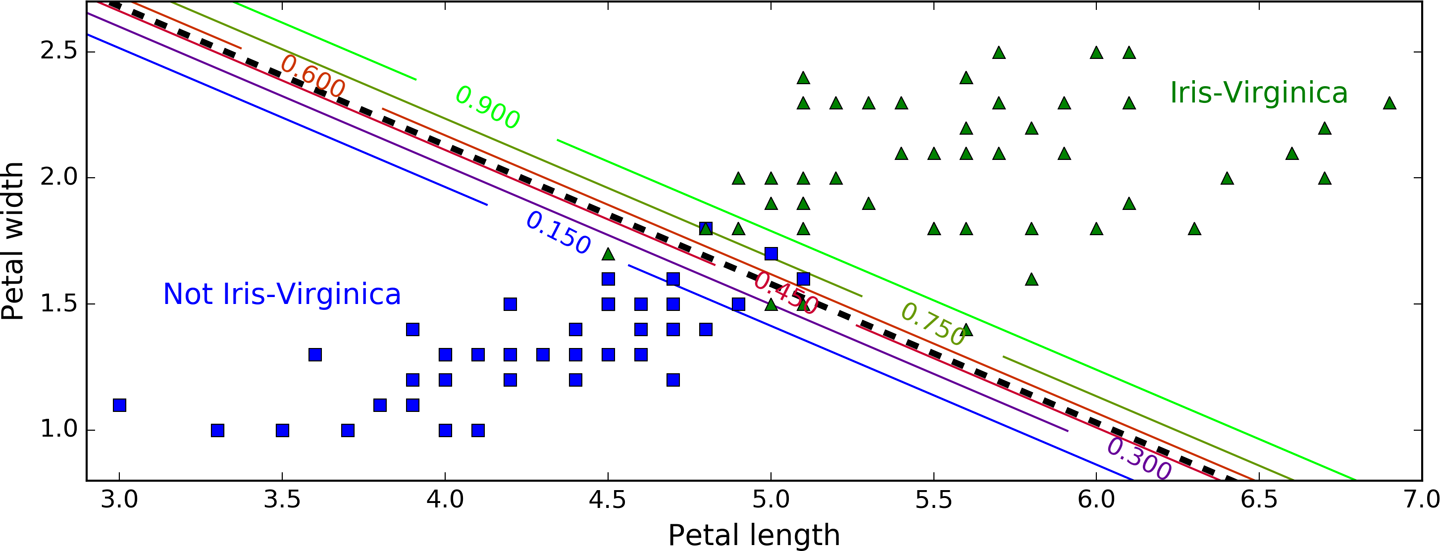
\includegraphics[width=\textwidth]{iris-2attr-decboundary.png}
{\vfill\footnotesize A. Géron, \emph{Hands-On Machine Learning with Scikit-Learn and TensorFlow} 2017}
\end{frame}

\begin{frame}{Funkcja logistyczna}
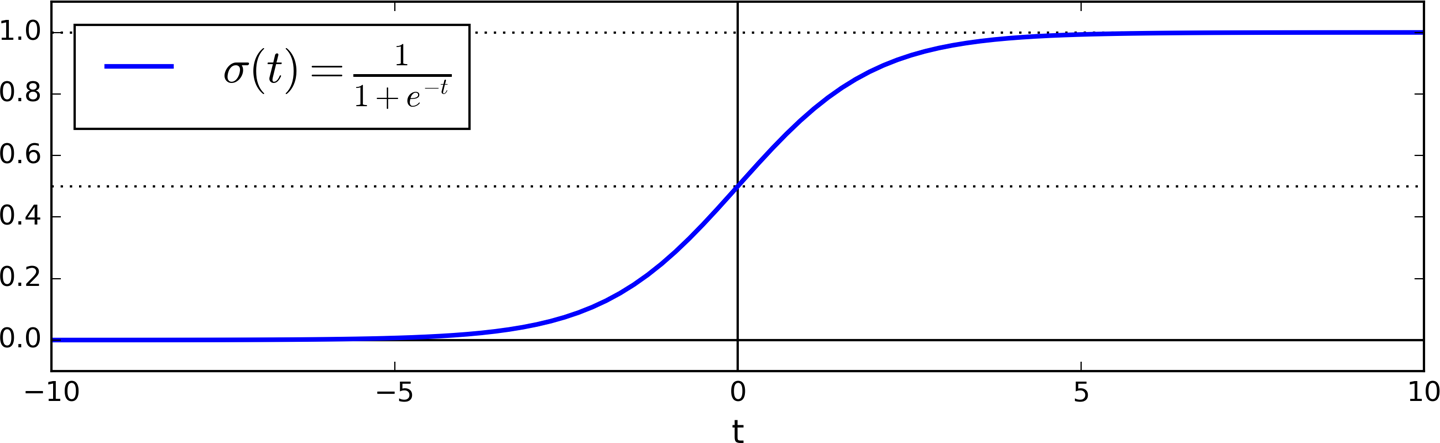
\includegraphics[width=\textwidth]{logistic-function.png}

{\vfill\footnotesize A. Géron, \emph{Hands-On Machine Learning with Scikit-Learn and TensorFlow} 2017}
\end{frame}

\begin{frame}{Pochodna funkcji logisytcznej}
\[ \sigma(t) = \frac{1}{1+e^{-t}} \]

\begin{block}{Zadanie}
Wiadomo, że $\sigma(t_0)=.1$. Czy da się na tej podstawie prosto obliczyć wartość pochodnej $\sigma'(t)$ w punkcie $t_0$?
\end{block}

\note{
\begin{gather*}
\sigma'(t)=-\left(\frac{1}{1+e^{-t}}\right)^2\cdot(-e^{-t})=\ldots=\sigma(t)(1-\sigma(t))
\end{gather*}
}
\end{frame}

\begin{frame}{Regresja logistyczna}
\begin{gather*}
\hat{p} = \sigma(\vec{x}\vec{w}) \\
\hat{y} = \begin{cases}
1 & \hat{p} \geq 0{,}5 \\
0 &\hat{p} < 0{,}5 \\
\end{cases}
\end{gather*}
\end{frame}

\begin{frame}{Funkcja kosztu dla pojedynczego przykładu}
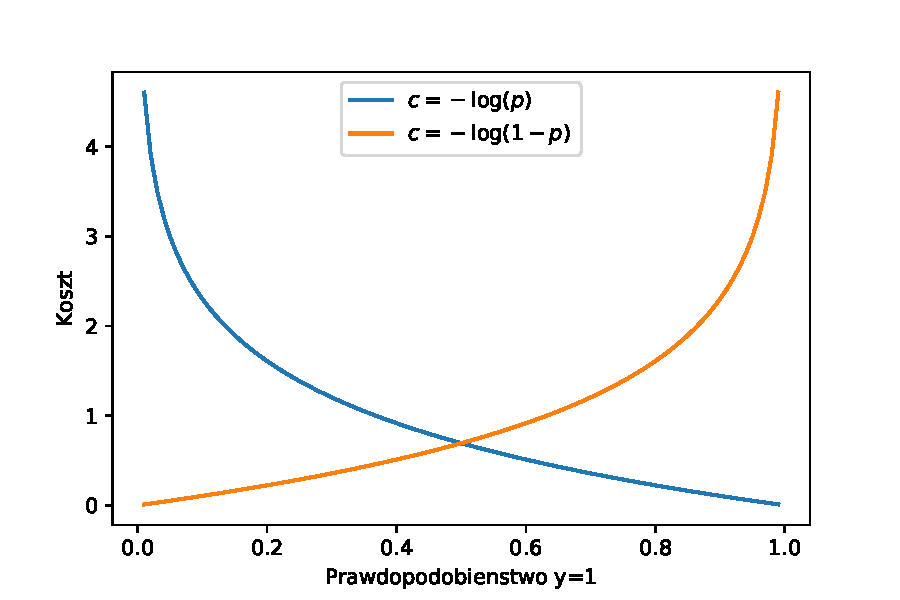
\includegraphics[width=\textwidth]{logreg-cost-single.pdf}
\end{frame}

\begin{frame}{Funkcja kosztu dla pojedynczego przykładu}
\begin{block}{Zadanie}
Zapisać poniższą funkcję jako pojedyncze wyrażenie (używając dodawania, mnożenia itp.):
\[ c(y, p) = \begin{cases} -\log(p) & y=1 \\ -\log(1-p) & y=0 \end{cases} \]
\end{block}
\note<1>
{
\[ c(y,p) = -y\log(p) - (1-y)\log(1-p) \]
}
\end{frame}

\begin{frame}{Funkcja kosztu dla całego problemu}
\begin{gather*}
\vec{p} = \sigma(\vec{X}\vec{w}) \\
J(\vec{w}) = \frac{1}{n} \sum_{i=1}^n c\left(y_i, p_i\right) = \\
-\frac{1}{n} \sum_{i=1}^n \left[ y_i\log p_i + (1-y_i)\log (1-p_i) \right] 
\end{gather*}
\pause
\[\frac{\dd J}{\dd w_i} = \frac{1}{n} \sum_{i=1}^n \left(\sigma(\vec{X_i}\vec{w})-y_i\right)X_{i,j} \]
\end{frame}

\begin{frame}{\emph{Softmax regression}/\emph{Multinomial logistic regression}}
\begin{block}{Zadanie klasyfikacji}
Dla danego wektora cech $x$ opisującego obiekt przewidzieć, do której z $K$ predefiniowanych klas należy obiekt: $y\in \{1, 2, \ldots, K\}$
\end{block}
% X n*p
% W p*k
\begin{gather*}
\vec{W} \text{ macierz wag typu } p\times k \\
\vec{P} \text{ macierz prawdopodobieństw typu } n\times k \\
\hat{\vec{P}} = \sigma(\vec{X}\vec{W}) = \left[ \frac{\sigma(\vec{X_{i,\cdot}}\vec{W_{\cdot,k}})}{\sum_{l=1}^K \sigma(\vec{X_{i,\cdot}}\vec{W_{\cdot,l}})} \right]_{i,k} \\
\hat{y_i} = \arg\max_{k} \hat{P_{i,k}} = \arg\max_{k} \vec{X_{i,\cdot}}\vec{W_{\cdot,k}} \\
\end{gather*}
\end{frame}

\begin{frame}{Uczenie regresji softmax}
\begin{gather*}
Y_{i,k}=\begin{cases} 1 & y_i=k \\ 0 & \text{w przeciwnym przypadku} \end{cases} \\
J(\vec{W}) = -\frac{1}{n} \sum_{i=1}^n \sum_{k=1}^K Y_{i,k}\log\hat{P_{i,k}} \\
\grad_{\vec{W_{\cdot,k}}} J(\vec{W}) = \frac{1}{n}\sum_{i=1}^n \left(\hat{P_{i,k}} - Y_{i,k}\right)\vec{X_{i}}
\end{gather*}
\end{frame}

\end{document}